\section{Example use-cases}\label{sec:tests}
As a case study for UNav-Sim, we present an autonomous pipe inspection scenario. 
%We have used pre-existing assets from the unreal engine marketplace to construct the simulation environment. This modular approach represents a straightforward and adaptable method for simulation environment construction.
Pipe inspection, being the most common use case for \ac{ROV}s, presents a relevant and challenging use case, where vision-based navigation is essential to achieve the required task. Furthermore, we assess the efficacy of our underwater autonomy stack and report its performance in executing the designated autonomous pipe inspection task. A video showing the pipe inspection demonstration can be found here\footnote{\url{https://youtu.be/unZS33lCqpU}}.



\subsection{Vision-based pipe following with DRL}\label{sec:example:planning}

In this experiment, the performance of UNav-Sim is evaluated in a pipe-following task. An agent utilizing \ac{DRL} is trained with the gym interface provided by the simulator to generate position commands based on RGB image observations. An \ac{MPC} controller subsequently executes the position commands. The convolutional neural network policy inputs $180\times320$ pixel RGB image observation, $o_t$, from a downward-looking camera on \ac{ROV} and outputs an action, $a_t$, describing one meter away waypoint consisting of two values, $a_1, a_2 \in [-1, 1]$. The actions represent the direction of the position step and turn in the heading angle, respectively, similar to our previous work \cite{halil}. The reward is defined with respect to vertical divergence from the pipe unless the termination of episodes; $r_t = 10 - 2e_p^2 - 2e_\psi$ where $e_p$ is the closest distance to the pipe in the horizontal plane and $e_\psi$ is the error in heading with respect to pipe direction. An episode is terminated where the pipes are not in the camera's field of view, which is $e_p > 2.5 m$. The \ac{DRL} agent is trained with proximal policy optimization~\cite{schulman2017proximal} algorithm using \texttt{stable-baselines3}~\cite{stable-baselines3} package.

The trained policy is deployed on a pipe $\sim20$ meters long with right and left turns. The trajectory of the agent along with the pipes is visualized in Fig. \ref{fig:trajectory_drl}.
While the agent is not accurately tracking the pipes due to the exploratory behavior of the \ac{DRL} policy, it learns to make reasoning from image observations and successfully follows the pipe.
This experiment demonstrates the utilization of high-fidelity image observations and accurate dynamics provided by UNav-Sim in a particular application.

\begin{figure}[t]
    \centering
    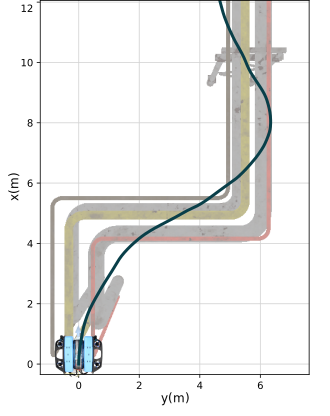
\includegraphics[width=8.4cm]{figs/paper5-unavsim/trajectory2.pdf}
    \caption[Trajectory drawn by the ROV in the DRL experiments]{Trajectory followed by the \ac{DRL} agent (dark blue) along with the pipes from the top view. The starting point is the origin of the coordinate frame and is indicated with the \ac{ROV}.
    %The  experimental results show that training the ego agent (\ac{ROV}) in a photo-realistic underwater environment can effectively enable it to be deployed in an underwater pipe inspection scenario.
    }
    \label{fig:trajectory_drl}
\end{figure}



\subsection{Visual localization benchmarking}
The vision-based trajectory generated in Section \ref{sec:example:planning}, being carried out by the robot with the controller showcased in Section \ref{sec:stack:control}, has served as a test setup for the visual localization experiment.
Two trajectories are carried out: a linear trajectory where no area in the map is revisited (see Fig. \ref{fig:trajectory_drl}), and a trajectory with a loop, where the robot navigates back to the starting point.
The benchmarking is automatically performed by the \texttt{robot\_visual\_localization} metapackage using \cite{grupp2017evo}. 

During runtime, the estimated trajectory $P_i$ and the ground truth trajectory $Q_i$ are recorded into separate files composing a sequence of time-synchronized spatial poses. The pose format is the one proposed in \cite{sturm2012tumrgbd}, composed of the three spatial coordinates with the orientation in quaternions.
The metrics implemented are the \ac{APE} and the \ac{RPE}, which are automatically deployed over the recorded trajectories before shutdown. TartanVO presents a monocular visual odometry algorithm. Therefore, for a fair comparison, the ORB-SLAM3 experiment is executed under a monocular setup. 
The deployment of monocular algorithms implies that the orientation of the algorithm's world frame and the trajectory's scale is arbitrary. Therefore, the estimated trajectories are aligned with the ground truth by obtaining the transform $S \in Sim_3$ that best aligns $P_i$ with $Q_i$.

With the deployment of the automatic stack for visual inspection proposed by UNav-Sim, benchmarking of visual localization algorithms becomes a straightforward task: the robot follows the pipeline autonomously under the planned trajectory, with the visual localization algorithms being automatically executed by the \texttt{robot\_visual\_localization} package, which on shutdown generates the results as depicted in Table \ref{unavsim:table:comparisonSLAM}. It can be seen from the generated results that the two proposed algorithms depict a similar performance in the linear trajectory, but ORB-SLAM outperforms TartanVO under the presence of a closed loop.
Despite ORB-SLAM's high efficiency in state-of-the-art datasets, the realistic underwater conditions confront one of the main challenges for feature-based approaches: the lack of texture. Moreover, the pipes are the main source of features, which avoids their uniform distribution across the image. Without enough evenly-distributed features, the ORB-SLAM's front end drifts. Nevertheless, the closed trajectory shows the convenience of the back-end's loop closure algorithm: the absolute errors are significantly reduced for translation and rotation.
On the other hand, TartanVO presents a drift similar to ORB-SLAM's in the translations, but slightly higher for rotations. These results show the great potential of learning-based algorithms under imaging conditions that challenge geometry-based methods. Although the lack of generalization ability is the main source of drift in this case, TartanVO has been trained with high amounts of diversified data that explain its good performance in the proposed setup.

In conclusion, the framework proposed in UNav-Sim has enabled the automatic benchmarking of state-of-the-art visual localisation algorithms in a realistic underwater scenario. This has allowed the challenges and opportunities of these algorithms to be easily demonstrated in a geometry-based and learning-based manner.

\begin{table}[ht!]
\centering
\footnotesize
\caption[Visual localization results in the pipeline tracking scenario]{Visual localization results in the pipeline tracking scenario.}
\label{unavsim:table:comparisonSLAM}
\begin{tabular}{cc c c c c  }
\toprule

Trajectory                   & Algorithm  & APE[m]         & RPE[m]         & APE[rad]       & RPE[rad] \\
\midrule
\multirow{2}{*}[0em]{Linear} & ORB-SLAM3  & 1.75          & \textbf{0.412} & \textbf{1.53} & \textbf{0.036} \\
                             & TartanVO   & \textbf{1.67} & 0.489          & 1.95          & 0.108 \\
\midrule
\multirow{2}{*}[0em]{With loop}   & ORB-SLAM3  & \textbf{0.078}          & 0.372 & \textbf{1.62} & \textbf{0.006} \\
                             & TartanVO   & 0.961 & \textbf{0.322}         & 2.10          & 0.068 \\
\bottomrule
\end{tabular}
\end{table}

% \begin{table}[ht!]
% \centering
% \scriptsize
% \caption{visual localization results in the pipeline tracking scenario.
% }
% \label{unavsim:table:comparisonSLAM}
% \begin{tabular}{|c| c c c c | }
% \hline

% Algorithm  & APE[m]         & RPE[m]         & APE[rad]       & RPE[rad] \\
% \hline
% ORB-SLAM3  & 1.754          & \textbf{0.412} & \textbf{1.525} & \textbf{0.036} \\
% TartanVO   & \textbf{1.667} & 0.489          & 1.952          & 0.108 \\
% \hline
% \end{tabular}
% \end{table}



